Assuming zone-relative spatio-temporal consensus, what is left is to make use of it for producing a verifiable \pol{} certificate. This section will provide a description of the certificate generation process, its requirements, and a possible verification procedure that is derived from the \pol{} protocol's design. 

Building upon the steps achieved in the previous sections, it is assumed that a zone has been established, and that the zone members are able to achieve time-conscious consensus. Concretely, we assume that both the prover and the witnesses restrict their communications to the zone's physical boundaries, dictated by the coverage of their short-ranged communication means, and we also assume that the zone members are able to achieve zone-relative time synchronization, and thus pace the events of the protocol's execution at the same rate. The next step is to establish the proof generation process, which is based on the zone's relative time and space. The higher goal is to assert that the prover is at a specific location, at a specific time, relative to the witnesses. This means, in practical terms, that the prover is able to communicate via the same short-ranged communication means with all the witnesses and is able to demonstrate that it is, as well, synchronized with their internal clocks. However, before asserting such propositions, we also assume that every entity $i$ has a unique key pair, composed of a public key $K^{pu}_i$ and a private key $K^{pr}_i$. The public key represents the identity of an entity and, therefore, is used to verify the signature of the messages sent by the entity. The private key, on the other hand, is used to sign the messages. The public key of a zone member is known to all the other members, meanwhile, the private keys are kept secret. 

Given that the witnesses $w \in W$ are pacing the zone events, i.e., generating new blocks, at every $T$ units of time, and the last block was generated at the zone-relative time $t_x$, with a block hash $h_x$, the proof generation process is as follows:

\begin{enumerate}
    \item The prover $\sigma$ synchronizes itself at the zone-relative time $t_x$ and learns the hash  $h_x$ of the last block $B_{x}$.
    \item The prover $\sigma$ assembles a transaction $\text{Tx}_\sigma$ containing the input $h_x$.
    \item The prover $\sigma$ signs the transaction $\text{Tx}_\sigma$ with its private key $K^{pr}_\sigma$.
    \item The prover $\sigma$ broadcasts the transaction $\text{Tx}_\sigma$ to the witnesses $w \in W$.
    \item The witnesses $w \in W$ verify the signature of the transaction $\text{Tx}_\sigma$.
    \item The witnesses $w \in W$ assemble a block $B_{x+1}$ with hash $h_{x+1}$, at time $t_{x+1}$, containing the transaction $\text{Tx}_\sigma$.
    \item The witnesses $w \in W$ sign the new block $B_{x+1}$ with their private key $K^{pr}_w$.
    \item The witnesses $w \in W$ broadcast the block $B_{x+1}$ to the entire network.
    \item The prover $\sigma$ verifies the hash $h_{x+1}$, the parent hash $h_{x}$, and the signatures of the block $B_{x+1}$, and the inclusion of its transaction $\text{Tx}_\sigma$, with the matching input $h_{x}$.
    \item The prover $\sigma$, finally, assembles the \pol{} certificate, containing the signed block $B_{x+1}$, by the witnesses $w \in W$, and the signed transaction $\text{Tx}_\sigma$, by the prover $\sigma$ itself.
\end{enumerate}

\begin{figure}[ht]
    \begin{center}
    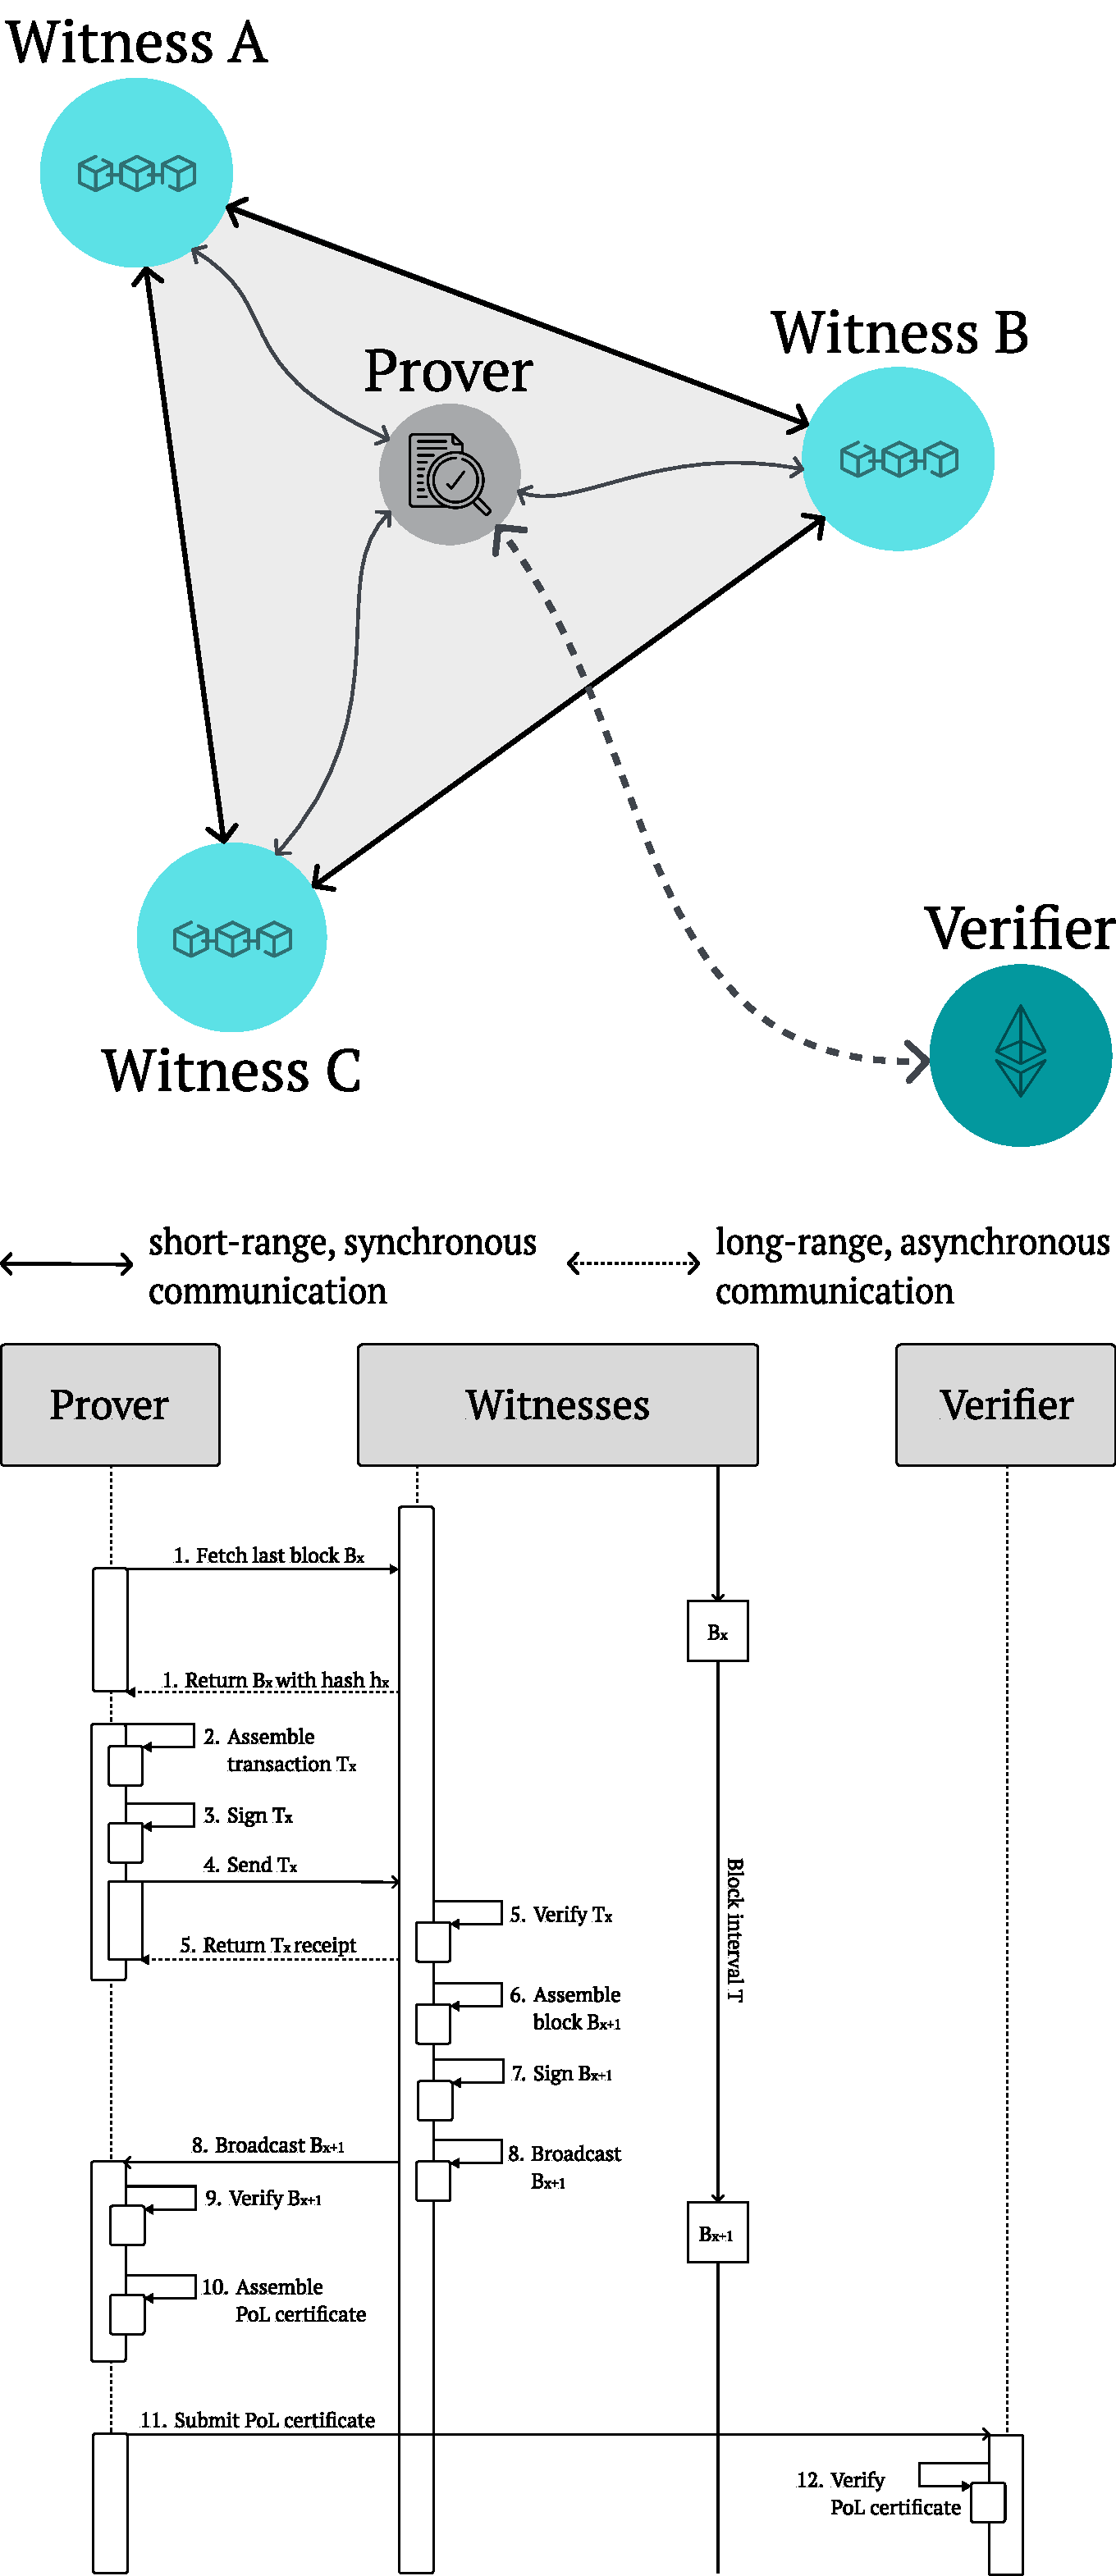
\includegraphics[width=\textwidth]{overview-pol-rel.pdf}
    \caption{Sequence diagram overview of the proof generation process.}
    \label{fig:proof-of-location-overview-relative-pol}
    \end{center}
\end{figure}

Having obtained a valid \pol{} certificate, as the prover $\sigma$ was spatially synchronized with the witnesses $w \in W$ around the zone-relative time $t_{x+1}$, the next step would be to submit the certificate to a verification process. Without any verifier-specific information, the verification process would be identical to step 9 of the above procedure. Assuming that the verifier knows the identities of all the entities involved in the proof generation process, the verification process would go around verifying the signatures of both the block $B_{x+1}$ and the transaction $\text{Tx}_\sigma$, by the witnesses and the prover, respectively, and verifying, as well, that the transaction input matches the parent hash $h_{x}$ of the block. This last verification step ensures that the prover was spatially synchronized with the witnesses around the zone-relative time $t_{x+1}$. A more well-founded analysis of the robustness, security, privacy, and, eventually, the correctness of this \pol{} protocol, as seen in the works presented in Chapter~\ref{sec:related-work}, is left for future work. This would, as well, include a more detailed analysis of the security against the most common attacks and collusion scenarios.

